% !Mode:: "TeX:UTF-8"% !TEX TS-program = xelatex
% !TEX encoding = UTF-8 Unicode
% !Mode:: "TeX:UTF-8"

%+++++++++++++++++++++++++++++++++++++++++++++++++++++++++++++++++++++++++++++
% This is a sample article script. All rights reserved.
% Author: qianhui@zju.edu.cn
%+++++++++++++++++++++++++++++++++++++++++++++++++++++++++++++++++++++++++++++
\documentclass[a4paper,twoside,AutoFakeBold]{article}
\usepackage{optreport}

%+++++++++++++++++++++++++++++++++++++++++++++++++++++++++++++++++++++++++++++
% Some packages for this sample.
%+++++++++++++++++++++++++++++++++++++++++++++++++++++++++++++++++++++++++++++
\usepackage{comment}	% Package for comment useless document
\usepackage{bm}			% Package for Bold-math symbol
\usepackage{mathrsfs}	% Package for RSFS fonts in maths
\usepackage{listings}	% Package for Listing code
\usepackage{enumerate}	% Package for enumerate
\usepackage{pdfrender}
\usepackage{subcaption}
\usepackage{multirow}
\usepackage{booktabs}
\usepackage{bbm}
\usepackage{bbding}
\usepackage{mathtools}
\usepackage{graphicx}
\usepackage{float}
\usepackage{epstopdf}
\usepackage{lipsum}
\usepackage{metalogo}
\usepackage{mdframed}

%+++++++++++++++++++++++++++++++++++++++++++++++++++++++++++++++++++++++++++++
% Title, Authors, Reprot Time.
%+++++++++++++++++++++++++++++++++++++++++++++++++++++++++++++++++++++++++++++
\serialnum{2024-2-0001}

\rptname{Optimal Transport Based Distributed \gaplongcap Optimization Research}

\rptauthora{周  楠}{3220102535} %作者1和学号
\rptauthorb{王晓宇}{3220104364} %作者2和学号
% \rptauthorc{张三丰}{109315043} %作者3和学号
\reporttime{2025}{1}

% -------------------------------------------------
% for english version.
% -------------------------------------------------
\rptcontentsname{Contents}
\renewcommand{\abstractname}{{\xiaosan Abstract}}
\def\bibetal{et al.}
\def\biband{and}
\makeatletter
\renewcommand*{\ALG@name}{{\xiaosi Algorithm.~}}
\makeatother
\theoremstyle{definition}
\newtheorem{defn2}{{Definition}}
\newtheorem{corr2}{{Corrollary}}[section]
\newtheorem{thrm2}{{Theorem}}[section]
\newtheorem{lema2}{{Lemma}}
\newtheorem{exmp2}{{Example}}[section]
\newtheorem{remark2}{{Remark}}
\renewcommand*{\proofname}{{\heiti Proof.~}}
\renewcommand{\figurename}{Fig.~}
\renewcommand{\tablename}{Tab.~}
\renewcommand{\refname}{Reference}
% -------------------------------------------------

%+++++++++++++++++++++++++++++++++++++++++++++++++++++++++++++++++++++++++++++
% Document.
%+++++++++++++++++++++++++++++++++++++++++++++++++++++++++++++++++++++++++++++
\begin{document}
\pagenumbering{gobble}

%-----------------------------------------------------------------------------
%  Title Page
%-----------------------------------------------------------------------------
\maketitle
\thispagestyle{empty} \clearpage

%-----------------------------------------------------------------------------
%  Table of Content
%-----------------------------------------------------------------------------
\rptcontent \thispagestyle{empty} \clearpage

%-----------------------------------------------------------------------------
%  Abstract
%-----------------------------------------------------------------------------
\begin{abstract}\kaiti \xiaosi
	We analyze Newton's method with lazy Hessian
	updates for solving general possibly non-convex
	optimization problems. We propose to reuse a
	previously seen Hessian for several iterations
	while computing new gradients at each step of
	the method. This significantly reduces the overall
	arithmetic complexity of second-order optimiza-
	tion schemes. By using the cubic regularization
	technique, we establish fast global convergence
	of our method to a second-order stationary point,
	while the Hessian does not need to be updated
	each iteration. For convex problems, we justify
	global and local superlinear rates for lazy New-
	ton steps with quadratic regularization, which is
	easier to compute. The optimal frequency for
	updating the Hessian is once every d iterations,
	where d is the dimension of the problem. This
	provably improves the total arithmetic complexity
	of second-order algorithms by a factor $\sqrt{d}$.

	\vspace{2em}  % 增加 2em 的垂直间距


	我们分析了用Lazy Hessian更新牛顿方法来解决一般的可能非凸优化问题。
	我们建议在方法的每一步计算新梯度的同时,在多次迭代中重复使用之前看到的 Hessian。
	这大大降低了二阶优化方案的整体算术复杂度。通过使用立方正则化技术,我们建立了我们的方法对二阶静止点的快速全局收敛性,
	同时不需要每次迭代更新Hessian。对于凸问题,我们证明了使用二次正则化的Lazy牛顿迭代法的全局和局部超线性率,这更容易计算。
	更新 Hessian 的最佳频率是每 d 次迭代一次,其中 d 是问题的维度。这可以证明,二阶算法的总算术复杂度提高了 $\sqrt{d}$ 倍。
\end{abstract}
\newpage
\clearpage

%-----------------------------------------------------------------------------
%  Sections
%-----------------------------------------------------------------------------
\pagenumbering{arabic}\songti\xiaosi
%-----------------------
%
%-----------------------
\section{论文研究的问题背景}
在优化问题中,二阶优化算法(如牛顿法)在处理条件不佳问题时表现出色,
尤其是在局部范围内能够达到快速的二次收敛速度。然而,牛顿法的全局收敛性依赖于初始点的选择,
且每一步都需要计算梯度和Hessian矩阵,并进行矩阵分解,计算成本较高。
特别是在大规模问题中,Hessian矩阵的计算和存储成本非常高,这限制了牛顿法在实际应用中的广泛使用。

本文的核心动机是减少二阶优化算法的计算复杂度,特别是减少Hessian矩阵的计算频率。
作者提出了一种简单但有效的方法:Lazy Hessian更新。
具体来说,算法在多次迭代中重用先前计算的Hessian矩阵,而每一步都使用新的梯度。
通过这种方式,可以显著减少Hessian矩阵的计算频率,从而降低总体的计算复杂度。

作者指出,Hessian矩阵的计算成本通常是梯度计算的d倍,其中d是问题的维度。
因此,通过减少Hessian矩阵的计算频率,可以显著加速算法的运行速度。
本文通过理论分析和实验验证,证明了Lazy Hessian更新方法在保持收敛速度的同时,能够显著减少计算成本。

\newpage

\section{论文的贡献}
\begin{enumerate}
    \item 提出了带有立方正则化的Lazy牛顿迭代法(第\Ref{sec:2}节):
	该方法在当前点计算梯度,而在过去的轨迹中使用Hessian矩阵。量化了二阶信息不精确性带来的误差,并形式化了单步方法的进展(定理\Ref{thrm:o2.1})。
	展示了如何通过按比例增加正则化参数来平衡$m$次连续Lazy牛顿迭代法的误差。
	
	\item 基于此,开发了带有Lazy Hessian的立方牛顿法(Algorithm \Ref{alg:1}),并证明了其快速全局收敛到二阶稳定点(第\Ref{sec:3}节的定理\Ref{thrm:3.1}):
	这避免了方法陷入鞍点的问题。当$m:=1$(每次迭代都更新Hessian矩阵)时,方法恢复为经典的立方牛顿法(Nesterov \& Polyak, 2006)。
	
	在考虑Hessian计算的实际算术成本的情况下,方法的最优选择是每$m:=d$次迭代更新一次Hessian矩阵,从而将立方牛顿法的总复杂度提高了
	$\sqrt{d}$倍(见推论\Ref{corr:3.6})。
	
	\item 展示了如何在问题是凸问题时改进方法(第\Ref{sec:4}节):
	开发了带有Lazy Hessian的正则化牛顿法(Algorithm \Ref{alg:2}),它将模型中的立方正则化替换为二次正则化。
	这使得子问题更容易求解,仅涉及一次标准的矩阵求逆,同时保持了原始立方正则化方法的快速收敛速度。
	
	\item 研究了新算法的局部收敛性(第\Ref{sec:5}节,见定理\Ref{thrm:5.1}和定理\Ref{thrm:5.3}):
	证明了这些算法都具有超线性收敛速度。作为一个特例,还证明了经典牛顿法(无正则化)在Lazy Hessian更新下的局部二次收敛性。
	
	\item 提供了数值实验:
	通过数值实验验证了所提出方法的有效性。
\end{enumerate}
\newpage

\section{论文的章节组织}

\begin{enumerate}
    \item Introduction(引言): 介绍了二阶优化算法的背景和动机,特别是牛顿法在处理病态问题时的优势及其计算成本高的局限性。
	提出了Lazy Hessian更新的核心思想,并概述了本文的主要贡献。
	\item Lazy Newton Steps(Lazy牛顿迭代法): 详细介绍了Lazy牛顿迭代法的定义和数学模型。通过在当前点计算梯度,
	而在过去的轨迹中使用Hessian矩阵,提出了带有立方正则化的Lazy牛顿迭代法。量化了二阶信息不精确性带来的误差,
	并形式化了单步方法的进展(定理\Ref{thrm:o2.1})。
	\item Global Convergence Rates(全局收敛性分析): 基于Lazy牛顿迭代法,提出了\textbf{带有Lazy Hessian的立方牛顿法(Algorithm \Ref{alg:2})}
	,并证明了其快速全局收敛到二阶稳定点(定理\Ref{thrm:3.1})。特别地,当Hessian每次迭代都更新时(\(m := 1\)),
	该方法恢复为经典的立方牛顿法。通过理论分析,证明了最优的Hessian更新频率是每\(d\)次迭代更新一次(\(m := d\)),
	从而将总复杂度提高了\(\sqrt{d}\)倍(推论\Ref{corr:3.6})。
	\item Minimizing Convex Functions(凸问题的优化): 针对凸问题,提出了\textbf{带有Lazy Hessian的正则化牛顿法(Algorithm \Ref{alg:2}},
	使用二次正则化替代立方正则化。这使得子问题更容易求解,仅涉及一次标准的矩阵求逆,同时保持了快速收敛速度。
	证明了该方法的全局复杂度与立方牛顿法相同,但每次迭代的计算成本更低。
	\item Local Superlinear Convergence(局部超线性收敛): 研究了新算法的局部收敛性,
	证明了这些算法在局部范围内具有超线性收敛速度(定理\Ref{thrm:5.1}和定理\Ref{thrm:5.3})。
	特别地,对于经典牛顿法(无正则化),在LazyHessian更新下也具有局部二次收敛性。
	\item Practical Implementation(实际实现): 讨论了算法的实际实现细节,包括矩阵分解和自适应搜索策略。
	提出了\textbf{自适应立方牛顿法(Algorithm \Ref{alg:3})},通过动态调整正则化参数来进一步提高算法的性能。
	\item Experiments(实验): 通过数值实验验证了所提出方法的有效性。实验包括Soft Maximum问题、Logistic回归问题和对角神经网络训练问题。
	结果表明,Lazy Hessian更新方法在保持收敛速度的同时显著减少了计算成本。
	\item Discussion(讨论): 总结了本文的主要贡献,并提出了未来可能的研究方向,包括研究具有特定Hessian结构的问题、
	探索LazyHessian更新与拟牛顿法之间的联系,以及将分析推广到高阶优化方案。
\end{enumerate}
\newpage

\section{论文的相关工作}

Lazy Hessian更新的思想并非全新,早在1967年,Shamanskii就提出了在非线性方程组求解中使用旧Hessian矩阵的局部收敛性分析。
Shamanskii证明了在更新Hessian矩阵时,迭代具有局部二次收敛速度,而在不更新Hessian矩阵时,迭代具有线性收敛速度。

此后,这一思想被广泛应用于各种正则化方法中,如Levenberg-Marquardt正则化、阻尼牛顿迭代法、近端牛顿法等。
这些方法通常具有渐近全局收敛性,但没有显式的非渐近收敛速度保证。

本文的工作与这些方法的不同之处在于,作者使用了现代全局化技术(如立方正则化和梯度正则化),
并证明了带有Lazy Hessian更新的二阶优化算法在广泛的凸和非凸优化问题中具有快速的全局收敛速度。特别是,本文提出了非渐近的全局复杂度保证,证明了LazyHessian更新方法在达到二阶稳定点时的全局复杂度为
$O(1/\epsilon^{3/2})$
同时显著减少了Hessian矩阵的计算频率。

此外,本文还与最近提出的分布式牛顿型方法进行了对比。这些方法在联邦学习等场景中使用了Hessian矩阵的概率聚合和压缩技术。
虽然这些方法也减少了Hessian矩阵的计算频率,但它们通常需要在每次迭代中评估Hessian矩阵,并根据某种准则决定是否使用新的Hessian矩阵。
相比之下,本文的方法在每$m$次迭代中只计算一次Hessian矩阵,从而进一步减少了计算成本。
\newpage

\section{论文的技术方法}


\subsection{问题描述和常用记号}

我们考虑以下优化问题:

\begin{equation}\label{1}
\min_{\mathbf{x} \in \mathbb{R}^d} f(\mathbf{x}), \tag{1}
\end{equation}

其中\(f\)是一个多次可微的函数,不一定是凸函数,我们假设其有下界:\(\inf_{\mathbf{x}} f(\mathbf{x}) \geq f^*\)。我们用\(\nabla f(\mathbf{x}) \in \mathbb{R}^d\)表示其梯度,用\(\nabla^2 f(\mathbf{x}) \in \mathbb{R}^{d \times d}\)表示其Hessian矩阵,计算于某个\(\mathbf{x} \in \mathbb{R}^d\)。

我们的分析既适用于标准的欧几里得空间,也适用于更一般的情况,即由任意固定的对称正定矩阵\(\mathbf{B} = \mathbf{B}^\top \succ 0\)定义的范数。在这种情况下,范数定义为

\begin{equation}\label{2}
\|\mathbf{x}\| \stackrel{\text{def}}{=} \left\langle \mathbf{B} \mathbf{x}, \mathbf{x} \right\rangle^{1/2}, \quad \mathbf{x} \in \mathbb{R}^d. \tag{2}
\end{equation}

因此,矩阵\(\mathbf{B}\)负责固定我们问题的坐标系。在最简单的情况下,我们可以选择\(\mathbf{B} := \mathbf{I}\)(单位矩阵),这恢复了经典的欧几里得几何。更高级的\(\mathbf{B}\)选择可以考虑问题的特定结构(见例3.2)。对偶对象(梯度)的范数以标准方式定义:

\[
\|\mathbf{g}\|_* \stackrel{\text{def}}{=} \sup_{\mathbf{x} : \|\mathbf{x}\| \leq 1} \left\langle \mathbf{g}, \mathbf{x} \right\rangle = \left\langle \mathbf{g}, \mathbf{B}^{-1} \mathbf{g} \right\rangle^{1/2}, \quad \mathbf{g} \in \mathbb{R}^d.
\]

矩阵\(\mathbf{A} \in \mathbb{R}^{d \times d}\)的诱导范数定义为

\[
\|\mathbf{A}\| \stackrel{\text{def}}{=} \sup_{\mathbf{x}, \mathbf{y} : \|\mathbf{x}\| \leq 1, \|\mathbf{y}\| \leq 1} \left\langle \mathbf{A} \mathbf{x}, \mathbf{y} \right\rangle = \sup_{\mathbf{x} : \|\mathbf{x}\| \leq 1} \|\mathbf{A} \mathbf{x}\|_*.
\]

我们假设\(f\)的Hessian是Lipschitz连续的,具有某个常数\(L > 0\):

\begin{equation}\label{3}
\|\nabla^2 f(\mathbf{x}) - \nabla^2 f(\mathbf{y})\| \leq L \|\mathbf{x} - \mathbf{y}\|, \quad \forall \mathbf{x}, \mathbf{y} \in \mathbb{R}^d. \tag{3}
\end{equation}
\newpage

\subsection{Lazy 牛顿迭代法}\label{sec:2}
Lazy牛顿迭代法的核心思想是重用先前计算的Hessian矩阵,而不是在每一步都重新计算。具体来说,算法在当前点计算梯度,而在过去的轨迹中使用Hessian矩阵。

Lazy牛顿迭代法的数学模型定义如下:
\[
Q_{\mathbf{x}, \mathbf{z}}(\mathbf{y}) = \langle \nabla f(\mathbf{x}), \mathbf{y} - \mathbf{x} \rangle + \frac{1}{2} \langle \nabla^{2}f(\mathbf{z})(\mathbf{y} - \mathbf{x}), \mathbf{y} - \mathbf{x} \rangle 
\]
\begin{equation}\label{4}
\mathbf{T}_{M}(\mathbf{x},\mathbf{z}) = \arg\min_{\mathbf{y}\in\mathbb{R}^{d}} 
\left\{ Q_{\mathbf{x}, \mathbf{z}}(\mathbf{y}) + \frac{M}{6} \|\mathbf{y} - \mathbf{x}\|^{3} \right\} \tag{4}
\end{equation}

\begin{itemize}
    \item \(\mathbf{x}\) 是当前点,\(\nabla f(\mathbf{x})\) 是在当前点计算的梯度。
    \item \(\mathbf{z}\) 是过去某次迭代的点,\(\nabla^{2}f(\mathbf{z})\) 是在该点计算的Hessian矩阵。
    \item \(M\) 是正则化参数,用于控制步长。
\end{itemize}

由于Hessian矩阵是过去某次迭代的计算结果,与当前点的Hessian矩阵可能存在差异,这种差异会引入误差。为了平衡这种误差,作者引入了\textbf{立方正则化},并通过增加正则化参数 \(M\) 来抵消误差的影响。

定义意味着点 \(\mathbf{T} = \mathbf{T}_{M}(\mathbf{x},\mathbf{z})\) 是立方正则化模型的全局最小值,尽管该模型通常是非凸的。然而,事实证明,可以使用最初为信任域方法开发的标准技术(Conn et al., 2000)高效地计算该点。

定义 \(r \stackrel{\text{def}}{=} \|\mathbf{T} - \mathbf{x}\|\)。\(\mathbf{T} = \mathbf{T}_{M}(\mathbf{x},\mathbf{z})\)的解满足以下平稳条件:

\[
\begin{cases}
\nabla f(\mathbf{x}) + \nabla^{2}f(\mathbf{z})(\mathbf{T} - \mathbf{x}) + \frac{M r}{2} \mathbf{B}(\mathbf{T} - \mathbf{x}) = \mathbf{0}, \\
\nabla^{2}f(\mathbf{z}) + \frac{M r}{2} \mathbf{B} \succeq 0.
\end{cases}
\]

因此,在非退化情况下,第一步可以表示为以下形式:

\begin{equation}\label{5}
\mathbf{T} = \mathbf{x} - \left( \nabla^{2}f(\mathbf{z}) + \frac{M r}{2} \mathbf{B} \right)^{-1} \nabla f(\mathbf{x}), \tag{5}
\end{equation}

并且可以通过求解相应的单变量非线性方程(Nesterov \& Polyak, 2006)找到值 \(r > 0\)。
这可以通过预先计算的Hessian矩阵的特征值或三对角分解非常高效地完成。通常,其成本与经典牛顿迭代法中的矩阵求逆相似。

定义以下量,对于 \(\mathbf{y} \in \mathbb{R}^{d}\):

\begin{equation}\label{6}
\xi(\mathbf{y}) \stackrel{\text{def}}{=} \left[ -\lambda_{\min} \left( \mathbf{B}^{-1/2} \nabla^{2}f(\mathbf{y}) \mathbf{B}^{-1/2} \right) \right]_{+}, \tag{6}
\end{equation}

其中 \([t]_{+} \stackrel{\text{def}}{=} \max\{t, 0\}\) 表示正部,\(\lambda_{\min}(\cdot)\) 是对称矩阵的最小特征值。如果对于某个 \(\mathbf{y} \in \mathbb{R}^{d}\) 有 \(\nabla^{2}f(\mathbf{y}) \succeq 0\),则 \(\xi(\mathbf{y}) = 0\)。否则,\(\xi(\mathbf{y})\) 表示Hessian矩阵的最小特征值相对于固定矩阵 \(\mathbf{B} \succ 0\) 的大小(绝对值)。

\begin{mdframed}
	

\begin{thrm2}\label{thrm:o2.1}
	
设 \(M \geq L\)。那么,对于一次立方步(\Ref{4}),有以下结论:
\begin{equation}\label{7}
f(\mathbf{x}) - f(\mathbf{T}) \geq \max \left\{ \frac{1}{648M^{2}} \xi(\mathbf{T})^{3}, 
\frac{1}{72\sqrt{2M}} \|\nabla f(\mathbf{T})\|_{*}^{3/2} \right\} + \frac{M}{48} r^{3} - \frac{11L^{3}}{M^{2}} \|\mathbf{z} - \mathbf{x}\|^{3}. \tag{7}
\end{equation}
\end{thrm2}
\end{mdframed}

定理\Ref{thrm:o2.1}展示了可以从一次带有立方正则化的Lazy牛顿迭代法中期望的进展。使用Lazy Hessian的代价是最后一项
,如果 \(\mathbf{z} := \mathbf{x}\)(为当前迭代更新Hessian矩阵),则该项消失。

\newpage

\subsection{全局收敛速率}\label{sec:3}

我们考虑算法的一个阶段,即我们在当前点\(\mathbf{z} := \mathbf{x}_0\)
计算一次Hessian矩阵,然后连续执行\(m\)次立方正则化步长(\Ref{4}):

\begin{equation}\label{8}
	\mathbf{x}_i = \mathbf{T}_M(\mathbf{x}_{i-1}, \mathbf{z}), \quad i = 1, \ldots, m. \tag{8}
\end{equation}


我们使用某个固定的正则化常数\(M > 0\)。从(\Ref{7})中可以看出,
使用旧的Hessian矩阵带来的误差与到起始点的距离的立方成正比:
\(\|\mathbf{x}_{i-1} - \mathbf{x}_0\|^3\) 对于每个 \(1 \leq i \leq m\)
我们这里可以通过选择一个足够大的
正则化参数\(M\)来平衡累积误差(\textit{accumulating error}),并同时聚合(\Ref{7})
中的正项。在这里,我们的目标是要保证下式成立:

\begin{equation}\label{9}
\frac{M}{48} \sum_{i=1}^{m} \|\mathbf{x}_i - \mathbf{x}_{i-1}\|^3 \geq 
\frac{11L^3}{M^2} \sum_{i=1}^{m} \|\mathbf{x}_{i-1} - \mathbf{x}_0\|^3.\tag{9}
\end{equation}

事实上,我们证明只需选择\(\boxed{M \geq 6mL}\)即可保证上式成立。{\color{blue}这里的证明我们
放到\Ref{sec:3.1}节证明。}


因此,我们能够处理(\Ref{8})中\(m\)次连续Lazy步长的累积误差。

在每次使用旧Hessian矩阵的立方步长(\Ref{8})内部阶段之后,我们在新的外部轮次中重新计算Hessian矩阵。
每个内部阶段的长度\(m \geq 1\)是算法的关键参数。为了方便表示,我们用\(\pi(k)\)表示小于或等于\(k\)的最大的\(m\)的倍数:

\begin{equation}\label{10}
\pi(k) \stackrel{\text{def}}{=} k - k \bmod m, \qquad k \geq 0. \tag{10}
\end{equation}

主算法定义如下,根据我们之前的分析,我们将使用一个简单的固定规则来选择正则化参数:

\begin{equation}\label{11}
\boxed{M := 6mL}. \tag{11}
\end{equation}

\begin{algorithm}[h]\xiaosi
	\caption{\xiaosi 带有Lazy Hessian的立方牛顿法}\label{alg:1}
	\begin{algorithmic} 
	\STATE 输入:\(\mathbf{x}_0 \in \mathbb{R}^d\),\(m \geq 1\),\(L > 0\), 选择\(M \geq 0\)。

	\STATE for \(k = 0, 1, \ldots\) do

	\STATE   设置最后一个快照点\(\mathbf{z}_k = \mathbf{x}_{\pi(k)}\)

	\STATE   计算Lazy立方步长\(\mathbf{x}_{k+1} = \mathbf{T}_M(\mathbf{x}_k, \mathbf{z}_k)\)
		
	\STATE end for

	\end{algorithmic}
\end{algorithm}

\begin{mdframed}

\begin{thrm2}\label{thrm:3.1}
	假设\(M\)如(1.4)所示固定。假设算法\Ref{alg:1}的
	前\(k\)次迭代的梯度高于所需的误差水平\(\varepsilon > 0\):	

\begin{equation}\label{12}
\|\nabla f(\mathbf{x}_i)\|_* \geq \varepsilon. \tag{12}
\end{equation}

那么,达到精度\(\|\nabla f(\mathbf{x}_{k+1})\|_* \leq \varepsilon\)所需的迭代次数最多为

\begin{equation}\label{13}
k \leq \mathcal{O}\left(\frac{\sqrt{mL}(f(\mathbf{x}_0) - f^*)}{\varepsilon^{3/2}}\right), \tag{13}
\end{equation}

在迭代期间,Hessian更新的总次数为

\begin{equation}\label{14}
t \leq \mathcal{O}\left(\frac{\sqrt{L}(f(\mathbf{x}_0) - f^*)}{\varepsilon^{3/2}\sqrt{m}}\right). \tag{14}
\end{equation}

对于所有Hessian矩阵的最小特征值,有

\begin{equation}\label{15}
\min_{1 \leq i \leq k} \xi(\mathbf{x}_i) \leq \mathcal{O}\left(\frac{M^2(f(\mathbf{x}_0) - f^*)}{k}\right)^{1/3}. \tag{15}
\end{equation}

\end{thrm2}

\end{mdframed}

假设所需的精度水平较小,即

\[
\varepsilon \leq \left(f(\mathbf{x}_0) - f^*\right)^{2/3} \left(\frac{L}{m}\right)^{1/3},
\]

这要求我们使用\textit{several Hessian}方法

为了选择参数\(m\),我们需要考虑算法所有迭代中实际所需的计算量。
我们用\textsl{GradCost}表示一次梯度步长的算术复杂度,
用\textsl{HessCost}表示计算Hessian矩阵及其适当分解的成本。一般来说,我们有

\begin{equation}\label{16}
\textsl{HessCost} = d \cdot \textsl{GradCost}, \tag{16}
\end{equation}

其中\(d\)是问题(\Ref{1})的维度。

\begin{exmp2}\label{exam:3.2}


设\(f(\mathbf{x}) = \frac{1}{n} \sum_{i=1}^{n} \phi((\mathbf{a}_i, \mathbf{x}))\),其中\(\mathbf{a}_i \in \mathbb{R}^d\),\(1 \leq i \leq n\)是给定的数据,\(\phi\)是固定的单变量光滑函数。在这种情况下,

\[
\nabla f(\mathbf{x}) = \mathbf{A}^\top \mathbf{s}(\mathbf{x}), \quad \text{且} \quad \nabla^2 f(\mathbf{x}) = \mathbf{A}^\top \mathbf{Q}(\mathbf{x}) \mathbf{A},
\]

其中\(\mathbf{A} \in \mathbb{R}^{n \times d}\)是以\(\mathbf{a}_1, \ldots, \mathbf{a}_n\)为行的矩阵;\(\mathbf{s}(\mathbf{x}) \in \mathbb{R}^n\)和\(\mathbf{Q}(\mathbf{x}) \in \mathbb{R}^{n \times n}\)是由下式给出的对角矩阵:

\[
\begin{bmatrix}
\mathbf{s}(\mathbf{x})
\end{bmatrix}_{(i)} \stackrel{\text{def}}{=} \frac{1}{n} \phi'((\mathbf{a}_i, \mathbf{x})),
\]
\[
\begin{bmatrix}
\mathbf{Q}(\mathbf{x})
\end{bmatrix}_{(i,i)} \stackrel{\text{def}}{=} \frac{1}{n} \phi''((\mathbf{a}_i, \mathbf{x})).
\]

由于Hessian矩阵的结构,使用矩阵\(\mathbf{B} := \mathbf{A}^\top \mathbf{A}\)来
定义我们的原始范数(即二范数)非常方便。实际上,对于这种范数的选择,我们可以证明
Hessian的Lipschitz常数仅依赖于损失函数\(\phi\)(即它是一个
绝对数值常数,不依赖于数据)。同时,当使用单位矩阵\(\mathbf{I}\)时,
相应的Lipschitz常数依赖于数据矩阵\(\|\mathbf{A}\|\)的大小。因此,
在后一种情况下,Lipschitz常数的值可能非常大。

假设计算\(\phi'(\cdot)\)和\(\phi''(\cdot)\)的成本为\(\mathcal{O}(1)\),且不依赖于问题参数。我们用\(\mathrm{nz}(\mathbf{A})\)表示矩阵\(\mathbf{A}\)的非零元素数量。那么,

\[
\textsl{HessCost} = \mathcal{O}\left( d \cdot \mathrm{nz}(\mathbf{A}) + d^3 \right),
\]

其中最后的三次项来自矩阵分解的计算(见\Ref{sec:3.2}矩阵分解),且

\[
\textsl{GradCost} = \mathcal{O}\left( \mathrm{nz}(\mathbf{A}) + d^2 \right),
\]

其中第二项来自使用分解。因此,关系(\Ref{16})成立。

\end{exmp2}


\begin{exmp2}\label{exam:3.3}

假设我们的目标函数由计算图表示(例如神经网络)。在这种情况下,
我们可以通过自动微分技术(Nocedal \& Wright, 2006)
计算Hessian-向量乘积\(\nabla^2 f(\mathbf{x}) \mathbf{h}\),
对于任何\(\mathbf{x}, \mathbf{h} \in \mathbb{R}^d\),
其成本与计算梯度\(\nabla f(\mathbf{x})\)相同。
因此,通常我们可以通过\(d\)次Hessian-向量乘积来计算Hessian矩阵,

\[
\nabla^2 f(\mathbf{x}) = \left[ \nabla^2 f(\mathbf{x}) \mathbf{e}_1 \mid \ldots \mid \nabla^2 f(\mathbf{x}) \mathbf{e}_d \right],
\]

其中\(\mathbf{e}_1, \ldots, \mathbf{e}_d\)是标准基向量。这满足(\Ref{16})。

\end{exmp2}	

\begin{exmp2}\label{exam:3.4}

对于任何可微函数,我们可以使用有限差分来近似其Hessian矩阵。
具体来说,对于固定参数\(\delta > 0\),我们可以形成
\(\mathbf{H}_{x,\delta} \in \mathbb{R}^{\delta \times d}\),其元素为

\[
\left[ \mathbf{H}_{x,\delta} \right]^{(i,j)} := \frac{1}{\delta} \left[ \nabla f(\mathbf{x} + \delta \mathbf{e}_i) - \nabla f(\mathbf{x}) \right]^{(j)},
\]

其中\(\mathbf{e}_1, \ldots, \mathbf{e}_d\)是标准基向量,
并使用以下对称化作为true\ Hessian的近似(见(Nocedal \& Wright, 2006; Cartis et al., 2012; Grapiglia et al., 2022)了解更多细节):

\[
\frac{1}{2} \left[ \mathbf{H}_{x,\delta} + \mathbf{H}_{x,\delta}^\top \right] \approx \nabla^2 f(\mathbf{x}).
\]

因此,形成Hessian近似需要\(d + 1\)次梯度计算,这与(\Ref{16})一致。

\end{exmp2}
根据定理\Ref{thrm:3.1},算法\Ref{alg:1}的总算术复杂度可以估计为

\begin{align}\label{17}
\text{Arithmetic Complexity} \\
&= k \times \text{GradCost} + t \times \text{HessCost} \\
&\stackrel{(1.6),(1.7),(1.9)}{\leq} \mathcal{O}\left( \left( \sqrt{m} + \frac{d}{\sqrt{m}} \right) \frac{\sqrt{L}(f(\mathbf{x}_0) - f^*)}{\varepsilon^{3/2}} \right)\\ 
&\times \textsl{GradCost}. \tag{17}
\end{align}

\begin{corr2}\label{corr:3.5}
对于\(\boxed{ m = 1} \),我们在每一步都更新Hessian矩阵。
这对应于完整的立方牛顿法(Nesterov \& Polyak, 2006),定理\Ref{thrm:3.1}恢复了其全局迭代复杂度:

\[
k = t \leq \mathcal{O}\left( \frac{\sqrt{L}(f(\mathbf{x}_0) - f^*)}{\varepsilon^{3/2}} \right).
\]

因此,该方法的总算术复杂度为

\begin{equation}\label{18}
\mathcal{O}\left( d \cdot \frac{\sqrt{L}(f(\mathbf{x}_0) - f^*)}{\varepsilon^{3/2}} \right) \cdot \textsl{GradCost}. \tag{18}
\end{equation}

\end{corr2}


\begin{corr2}\label{corr:3.6}
	
对于\(\boxed{ m = d}\),我们得到了一个阶段的最优选择,它最小化了(\Ref{17}7)的右侧。算法\Ref{alg:1}的总算术复杂度变为

\[
\mathcal{O}\left( \sqrt{d} \cdot \frac{\sqrt{L}(f(\mathbf{x}_0) - f^*)}{\varepsilon^{3/2}} \right) \cdot \text{GradCost}.
\]

这比完整的立方牛顿法提高了\(\sqrt{d}\)倍。

现在,我们可以查看算法生成的所有Hessian矩阵的最小特征值。

\end{corr2}

\begin{corr2}\label{corr:3.7}
固定某个\(\varepsilon > 0\),

\begin{equation}\label{19}
k = \frac{\sqrt{mL}(f(\mathbf{x}_0) - f^*)}{\varepsilon^{3/2}} \tag{19}
\end{equation}

并执行\(k\)次算法\Ref{alg:1}的迭代。根据定理\Ref{thrm:3.1},我们因此确保\(\min_{1 \leq i \leq k} \|\nabla f(\mathbf{x}_i)\|_* \leq \mathcal{O}(\varepsilon)\)。同时,

\[
\min_{1 \leq i \leq k} \xi(\mathbf{x}_i) \stackrel{(\Ref{15})}{\leq} \left( \frac{648M^2(f(\mathbf{x}_0) - f^*)}{k} \right)^{1/3} \stackrel{(\Ref{19})}{\cong} 2^{5/3} 3^2 \sqrt{mL\varepsilon} .
\]

因此,Hessian矩阵的负特征值不会太大。对于\(\mathcal{O}(\varepsilon)\)级别的
梯度范数,我们保证最小特征值(\Ref{6})的级别为\(\mathcal{O}(\sqrt{mL} \varepsilon)\)。

\end{corr2}


\subsubsection{\(M \geq 6mL\)取法的证明}\label{sec:3.1}

我们用\(r_{k+1} := \|\mathbf{x}_{k+1} - \mathbf{x}_k\|\)表示相应的步长。
根据定理\Ref{thrm:o2.1},对于每个\(0 \leq k \leq m-1\),我们有以下关于目标函数的不等式:

\begin{align}
f(\mathbf{x}_k) - f(\mathbf{x}_{k+1}) \\
&\geq \max \left\{ \frac{1}{648M^2} \xi(\mathbf{x}_{k+1})^3, \frac{1}{72\sqrt{2M}} \|\nabla f(\mathbf{x}_{k+1})\|_*^{3/2} \right\} \\
&+ \frac{M}{48} r_{k+1}^3 - \frac{11L^3}{M^2} \|\mathbf{x}_0 - \mathbf{x}_k\|^3. 
\end{align}

将这个不等式对不同的\(k\)进行累加,并使用最后一个负项的三角不等式,

\[
\|\mathbf{x}_0 - \mathbf{x}_k\| \leq \sum_{i=1}^{k} r_i,
\]

我们得到

\begin{align}\label{B.47}
f(\mathbf{x}_0) - f(\mathbf{x}_m) \\
&\geq \sum_{k=1}^{m} \max \left\{ \frac{1}{648M^2} \xi(\mathbf{x}_k)^3, \frac{1}{72\sqrt{2M}} \sum_{k=1}^{m} \|\nabla f(\mathbf{x}_k)\|_*^{3/2} \right\} \\
&+ \frac{M}{48} \sum_{k=1}^{m} r_k^3 - \frac{11L^3}{M^2} \sum_{k=1}^{m-1} \left( \sum_{i=1}^{k} r_i \right)^3. \tag{B.47}
\end{align}

接下来,我们使用以下简单的引理。

\begin{lema2}\label{lema:B.48}
对于任何正数序列\(\{r_k\}_{k \geq 1}\),对于任何\(m \geq 1\),有

\[
\sum_{k=1}^{m-1} \left( \sum_{i=1}^{k} r_i \right)^3 \leq \frac{m^3}{3} \sum_{k=1}^{m-1} r_k^3. \tag{B.48}
\]
\end{lema2}

\begin{proof}
引理证明如下。

我们通过归纳法证明(\Ref{lema:B.48})。对于\(m = 1\),显然成立,这是我们的归纳奠基。

假设对于某个任意的\(m \geq 1\)成立。那么

\begin{equation}\label{B.49}
\sum_{k=1}^{m} \left( \sum_{i=1}^{k} r_i \right)^3 = 
\sum_{k=1}^{m-1} \left( \sum_{i=1}^{k} r_i \right)^3 + 
\left( \sum_{i=1}^{m} r_i \right)^3 \leq \frac{48}{3} 
\sum_{k=1}^{m-1} r_k^3 + \left( \sum_{i=1}^{m} r_i \right)^3. \tag{B.49}
\end{equation}

对第二个项应用凸函数\(t \mapsto t^3\)的Jensen不等式,我们得到

\begin{equation}\label{B.50}
\left( \sum_{i=1}^{m} r_i \right)^3 = m^3 \left( \frac{1}{m} 
\sum_{i=1}^{m} r_i \right)^3 \leq m^2 \sum_{i=1}^{m} r_i^3. \tag{B.50}
\end{equation}

因此,

\[
\sum_{k=1}^{m} \left( \sum_{i=1}^{k} r_i \right)^3 \leq 
\left( \frac{m^3}{3} + m^2 \right) \sum_{k=1}^{m} r_k^3 
\leq \frac{(m+1)^3}{3} \sum_{k=1}^{m} r_k^3. 
\]
\end{proof}
使用这个不等式,我们确保(\Ref{B.47})的右侧为正。为此,我们需要使用一个增加的正则化参数值。因此,我们证明了以下保证。

\begin{corr2}\label{corr:B.2}
设\(M \geq 6mL\)。那么,

\begin{equation}\label{B.51}
f(\mathbf{x}_0) - f(\mathbf{x}_m) \geq \sum_{k=1}^{m} 
\max \left\{ \frac{1}{648M^2} \xi(\mathbf{x}_k)^3, \frac{1}{72\sqrt{2M}} 
\|\nabla f(\mathbf{x}_k)\|_*^{3/2} \right\}. \tag{B.51}
\end{equation}

\end{corr2}

\begin{thrm2}\label{thrm:B.3}
假设目标函数有下界:\(\inf_{\mathbf{x}} f(\mathbf{x}) \geq f^*\)。设正则化参数\(M\)如(\Ref{11})所示固定。
假设算法\Ref{alg:1}的前\(k\)次迭代的梯度高于所需的误差水平\(\varepsilon > 0\):

\begin{equation}\label{B.52}
\|\nabla f(\mathbf{x}_i)\|_* \geq \varepsilon. \tag{B.52}
\end{equation}

那么,达到精度\(\|\nabla f(\mathbf{x}_{k+1})\|_* \leq \varepsilon\)所需的迭代次数最多为

\begin{equation}\label{B.53}
k \leq \mathcal{O}\left( \frac{\sqrt{mL}(f(\mathbf{x}_0) - f^*)}{\varepsilon^{3/2}} \right), \tag{B.53}
\end{equation}

其中\(\mathcal{O}(\cdot)\)隐藏了一些绝对数值常数。在这些迭代期间,Hessian更新的总次数\(t\)满足

\begin{equation}\label{B.54}
t \leq \mathcal{O}\left( \frac{\sqrt{L}(f(\mathbf{x}_0) - f^*)}{\varepsilon^{3/2}\sqrt{m}} \right). \tag{B.54}
\end{equation}

对于所有Hessian矩阵的最小特征值,有

\begin{equation}\label{B.55}
\min_{1 \leq i \leq k} \left[ -\lambda_{\min} \left( \mathbf{B}^{-1/2} \nabla^2 f(\mathbf{x}_i) \mathbf{B}^{-1/2} \right) \right]_+ 
\leq \left( \frac{648M^2(f(\mathbf{x}_0) - f^*)}{k} \right)^{1/3}. \tag{B.55}
\end{equation}

\end{thrm2}

\begin{proof}
不失一般性,我们假设\(k\)是\(m\)的倍数:\(k = tm\)。那么,对于方法的第\(i\)个阶段(\(1 \leq i \leq t\)),我们有

\begin{equation}\label{B.56}
f(\mathbf{x}_{m(i-1)}) - f(\mathbf{x}_{mi}) \geq \frac{m}{72\sqrt{2M}} \varepsilon^{3/2} = \frac{\sqrt{m}}{144\sqrt{3L}} \varepsilon^{3/2}. \tag{B.56}
\end{equation}

对所有阶段进行累加,我们得到

\begin{equation}\label{B.57}
f(\mathbf{x}_0) - f^* \geq f(\mathbf{x}_0) - f(\mathbf{x}_k) \geq \frac{t\sqrt{m}}{144\sqrt{3L}} \varepsilon^{3/2}. \tag{B.57}
\end{equation}

这给出了\(t\)的所需上界(\Ref{14})。考虑到\(k = tm\),(\Ref{B.53})立即成立。对于Hessian矩阵的最小特征值\(\xi(\cdot)\),累加(\Ref{B.51})得到

\begin{equation}\label{B.58}
f(\mathbf{x}_0) - f^* \geq f(\mathbf{x}_0) - f(\mathbf{x}_k) \geq \frac{k}{648M^2} \min_{1 \leq i \leq k} \xi(\mathbf{x}_i)^3. \tag{B.58}
\end{equation}

因此,

\[
\min_{1 \leq i \leq k} \left[ -\lambda_{\min} \left( \mathbf{B}^{-1/2} \nabla^2 f(\mathbf{x}_i) \mathbf{B}^{-1/2} \right) \right]_+ 
\equiv \min_{1 \leq i \leq k} \xi(\mathbf{x}_i) \leq \left( \frac{648M^2(f(\mathbf{x}_0) - f^*)}{k} \right)^{1/3},
\]

\end{proof}

\subsubsection{矩阵分解}\label{sec:3.2}

在每\(m\)次迭代计算一次Hessian矩阵后,我们希望能够在方法的每次迭代中高效地解决相应的子问题。

为了求解立方牛顿法(\Ref{4})中的子问题,我们需要找到参数\(r > 0\),在非退化情况下,它是以下非线性方程的根(见Nesterov \& Polyak, 2006):

\begin{equation}\label{24}
\varphi(r) \stackrel{\text{def}}{=} \|\mathbf{s}(r)\| - r = 0, \tag{24}
\end{equation}

其中\(\mathbf{s}(r) \stackrel{\text{def}}{=} \left( \nabla^2 f(\mathbf{z}) + \frac{M r}{2} \mathbf{B} \right)^{-1} \nabla f(\mathbf{x})\),
对于使得矩阵正定的\(r\)。对(\Ref{24})应用标准的二分法或单变量牛顿法(步长为\(r^+ = r - \varphi(r)/\varphi'(r)\)),
我们需要执行的主要操作是求解线性方程:

\begin{equation}\label{25}
\left( \nabla^2 f(\mathbf{z}) + \tau \mathbf{B} \right) \mathbf{h} = -\nabla f(\mathbf{x}), \tag{25}
\end{equation}

对于不同的\(\tau > 0\)。这与我们在算法\Ref{alg:2}中每次迭代需要执行的操作类型相同。

现在,假设我们有以下Hessian矩阵的分解:

\begin{equation}\label{26}
\nabla^2 f(\mathbf{z}) = \mathbf{U} \boldsymbol{\Lambda} \mathbf{U}^\top, \quad \text{其中} \quad \mathbf{U} \mathbf{U}^\top = \mathbf{B}, \tag{26}
\end{equation}

且\(\boldsymbol{\Lambda} \in \mathbb{R}^{d \times d}\)是一个\textbf{对角}或\textbf{三对角}矩阵。因此,\(\mathbf{U}\)是关于\(\mathbf{B}\)正交的一组向量。
在\(\mathbf{B} = \mathbf{I}\)(单位矩阵)且\(\boldsymbol{\Lambda}\)为对角矩阵的情况下,(\Ref{26})被称为\textbf{特征值分解},并在大多数标准线性代数库中实现。

一般来说,分解(\Ref{26})可以在\(\mathcal{O}(d^3)\)次算术操作中计算。具体来说,我们可以对以下矩阵应用标准的正交化分解:

\[
\mathbf{B}^{-1/2} \nabla^2 f(\mathbf{z}) \mathbf{B}^{-1/2} = \mathbf{V} \boldsymbol{\Lambda} \mathbf{V}^\top, \quad \text{其中} \quad \mathbf{V} \mathbf{V}^\top = \mathbf{I},
\]

然后设\(\mathbf{U} := \mathbf{B}^{1/2} \mathbf{V}\),得到(\Ref{26})。注意,(\Ref{25})的解可以表示为

\[
\mathbf{h} = -\mathbf{U}^{-\top} \left( \boldsymbol{\Lambda} + \tau \mathbf{I} \right)^{-1} \mathbf{U}^{-1} \nabla f(\mathbf{x}),
\]

对于任何给定的\(\tau > 0\)和\(\nabla f(\mathbf{x})\),它可以在\(\mathcal{O}(d^2)\)次算术操作中计算。使用三对角分解在实践中可能更高效。
实际上,对于三对角矩阵\(\boldsymbol{\Lambda}\),矩阵\(\boldsymbol{\Lambda} + \tau \mathbf{I}\)的逆运算仍然只需要\(\mathcal{O}(d)\)次操作,
而计算这种分解所需的计算资源和浮点精度较少。在实践中,利用Hessian矩阵的结构(例如矩阵是稀疏的)也可以进一步减少每一步的算术成本。


\newpage

\subsection{凸问题的优化}\label{sec:4}
在凸优化问题中,目标函数的Hessian矩阵是半正定的(即 \(\nabla^{2}f(\mathbf{x}) \succeq 0\))。
这使得可以使用更简单的正则化技术来简化子问题的求解。本文针对凸问题,提出了
\textbf{带有LazyHessian的正则化牛顿法(Algorithm 2)},使用二次正则化替代立方正则化,从而使得子问题更容易求解。

\begin{algorithm}
\caption{Regularized Newton with Lazy Hessians}\label{alg:2}
\begin{algorithmic}[2]
\REQUIRE $\mathbf{x}_{0} \in \mathbb{R}^{d}$, $m \geq 1$, $L > 0$
\ENSURE Sequence $\{\mathbf{x}_{k}\}_{k \geq 0}$ converging to a second-order stationary point

\STATE Choose $M := 3mL$ \COMMENT{Set regularization parameter}
\FOR{$k = 0, 1, \ldots$}
	\STATE Set last snapshot point $\mathbf{z}_{k} = \mathbf{x}_{\pi(k)}$ \COMMENT{Reuse Hessian from $\pi(k)$-th iteration}
	\STATE Compute $\lambda_{k} = \sqrt{M \|\nabla f(\mathbf{x}_{k})\|_{*}}$ \COMMENT{Compute regularization parameter}
	\STATE Compute lazy Newton step:
	\[
	\mathbf{x}_{k+1} = \mathbf{x}_{k} - \left( \nabla^{2}f(\mathbf{z}_{k}) + \lambda_{k} \mathbf{B} \right)^{-1} \nabla f(\mathbf{x}_{k})
	\]
\ENDFOR
\end{algorithmic}
\end{algorithm}
算法\Ref{alg:2}的全局复杂度界与算法\Ref{alg:1}的复杂度界相同(最多相差一个对数项)。然而,算法\Ref{alg:2}的每次迭代更容易实现,因为它仅涉及求解一个线性系统。
\begin{mdframed}
	\begin{equation}\label{20}
		M := 3mL , \tag{20}
	\end{equation}
\end{mdframed}
\begin{itemize}
    \item \textbf{迭代次数}:达到精度 \(\|\nabla f(\mathbf{x}_{k+1})\|_{*} \leq \varepsilon\) 所需的迭代次数为:
    \begin{equation}\label{22}
    k \leq \mathcal{O}\left( \frac{\sqrt{m} L (f(\mathbf{x}_{0}) - f^{*})}{\varepsilon^{3/2}} + \ln \frac{\|\nabla f(\mathbf{x}_{0})\|_{*}}{\varepsilon} \right). \tag{22}
	\end{equation}

    \item \textbf{Hessian更新次数}:在达到精度 \(\varepsilon\) 的过程中,Hessian矩阵的更新次数为:
    \begin{equation}\label{23}
    t \leq \mathcal{O}\left( \frac{\sqrt{L} (f(\mathbf{x}_{0}) - f^{*})}{\varepsilon^{3/2} \sqrt{m}} + \frac{1}{m} \ln \frac{\|\nabla f(\mathbf{x}_{0})\|_{*}}{\varepsilon} \right). \tag{23}
    \end{equation}
\end{itemize}
\newpage

\subsection{局部超线性收敛证明(强凸函数)}\label{sec:5}


在本节中,我们讨论了带有Lazy\ Hessian更新的二阶优化算法的局部收敛性。我们展示了在每个阶段内具有恒定因子的快速线性收敛速率,并考虑了Hessian更新后的超线性收敛。

假设我们的目标是\textbf{强凸}的,即\(\nabla^2 f(\mathbf{x}) \succeq \mu \mathbf{B}, \forall \mathbf{x} \in \mathbb{R}^d\),其中\(\mu > 0\)是强凸参数。为了简化分析,我们要求在整个空间中的所有点都满足强凸性,尽管也可以在解的邻域内分析牛顿迭代法长的强凸性。

\begin{mdframed}
\begin{thrm2}\label{thrm:5.1}
设\(M \geq 0\)。假设初始梯度足够小:\(\|\nabla f(\mathbf{x}_0)\|_* \leq \frac{1}{2} \mathcal{G}_0\),
其中\(\mathcal{G}_0 := \frac{\mu^2}{3L + M}\)。那么,算法\Ref{alg:1}在梯度范数上具有超线性收敛性,对于\(k \geq 0\):

\[
\|\nabla f(\mathbf{x}_k)\|_* \leq \mathcal{G}_0 \cdot \left( \frac{1}{2} \right)^{(1 + m)^{\pi(k)} (1 + k \bmod m)},
\]

其中\(\pi(k)\)由规定术语(\Ref{10})定义。
\end{thrm2}
\end{mdframed}

\begin{corr2}\label{corr:5.2}
结合定理\Ref{thrm:3.1}和定理\Ref{thrm:5.1},我们得出结论:对于使用正则化参数\(M\)如(\Ref{11})
所示的算法\Ref{alg:1},从任意\(\mathbf{x}_0\)开始,最小化强凸函数所需的Lazy步长次数为

\[
k \leq \mathcal{O}\left( \frac{m^2 L^2 (f(\mathbf{x}_0) - f^*)}{\mu^3} + \frac{1}{\ln(1 + m)} \ln \ln \frac{\mu^2}{m L \varepsilon} \right),
\]

以达到\(\|\nabla f(\mathbf{x}_k)\|_* \leq \varepsilon\)。

我们还展示了算法\Ref{alg:2}在局部具有稍差但仍然超线性的收敛速率,
这在实践中已经非常快了。例如,对于\(m = 1\),算法2具有阶数为\(3/2\)的
超线性收敛速率,而算法\Ref{alg:1}的阶数为\(2\)。
\end{corr2}

\begin{mdframed}
\begin{thrm2}\label{thrm:5.3}
设\(M \geq 0\)。假设初始梯度足够小:\(\|\nabla f(\mathbf{x}_0)\|_* \leq \frac{1}{2^2} \mathcal{G}_0\),
其中\(\mathcal{G}_0 := \frac{\mu^2}{2^3 (3L + 4M)}\)。那么,算法\Ref{alg:2}在梯度范数上具有超线性收敛性,对于\(k \geq 0\):

\[
\|\nabla f(\mathbf{x}_k)\|_* \leq \mathcal{G}_0 \cdot \left( \frac{1}{2} \right)^{2(1 + m/2)^{\pi(k)}(1 + (k \bmod m)/2)} ,
\]

其中\(\pi(k)\)由(\Ref{10})定义。
\end{thrm2}
\end{mdframed}

\begin{corr2}\label{corr:5.4}
结合定理\Ref{sec:4}和定理\Ref{thrm:5.3},我们得出结论:对于使用
正则化参数\(M\)如(\Ref{20})所示的算法\Ref{alg:2},从任意
\(\mathbf{x}_0\)开始,最小化强凸函数所需的Lazy步长次数为

\[
k \leq \mathcal{O}\left( \frac{m^2 L^2 (f(\mathbf{x}_0) - f^*)}{\mu^3} + \ln \frac{m L \|\nabla f(\mathbf{x}_0)\|_*}{\mu^2} + \frac{1}{\ln(1 + m/2)} \ln \ln \frac{\mu^2}{m L \varepsilon} \right),
\]

以达到\(\|\nabla f(\mathbf{x}_k)\|_* \leq \varepsilon\)。
\end{corr2}
\newpage

\subsection{实践实现之自适应搜索}\label{sec:6}
\textsl{前一小节的矩阵分解已经在全局收敛速率处提到,这里便不再赘述,只说明自适应搜索的实践实现。}

为了得到我们的结果,我们需要选择正则化参数\(M\)与\(mL\)成正比,其中\(m \geq 1\)是一个阶段的长度,
\(L > 0\)是Hessian的Lipschitz常数。这种选择的一个缺点是,我们实际上需要知道Lipschitz常数,
而这在实践中并不总是可行的。此外,使用固定的正则化参数会使方法变得保守,阻止了大步长的可能性。
同时,从局部角度来看,目标函数的最佳二次近似是纯二阶泰勒多项式。因此,在解的邻域内,
最佳策略是使\(M\)趋近于零,从而获得最快的局部超线性收敛速率(见章节\Ref{sec:5})。

在二阶优化算法中使用自适应搜索已经研究了多年(Nesterov \& Polyak, 2006; Cartis et al., 2011a,b; Grapiglia \& Nesterov, 2017, 2019; Doikov \& Nesterov, 2021a,b)。
众所周知,这种方案在实际中表现非常好,同时自适应搜索使方法具有\textbf{通用性}(Grapiglia \& Nesterov, 2017; Doikov \& Nesterov, 2021a),
即能够适应Hessian的最佳Hölder度,甚至\textbf{超通用性}(Doikov et al., 2022),
即自动选择目标函数的二阶或三阶导数的Hölder度,从而在广泛的问题类上具有最佳的全局复杂度保证。

我们提出了算法\Ref{alg:3},它自适应地改变\(M\)的值,并在\(m\)步后检查函数进展以验证其选择。
重要的是,不需要知道Lipschitz常数\(L\)。

\begin{algorithm}
	\caption{带有Lazy Hessian的自适应立方牛顿法}\label{alg:3}
	\begin{algorithmic}[2]
	\REQUIRE $\mathbf{x}_0 \in \mathbb{R}^d$,$m \geq 1$。固定某个$M_0 > 0$。
		\FOR {$t = 0, 1, \ldots$} 
			\STATE 计算快照Hessian $\nabla^2 f(\mathbf{x}_{tm})$
			\STATE 更新$M_t = 2 \cdot M_t$
			\FOR {$i = 1, \ldots, m$}
				\STATE Lazy 立方步长 $\mathbf{x}_{tm + i} = T_{M_t}(\mathbf{x}_{tm + i - 1}, \mathbf{x}_{tm})$
			\ENDFOR
			\IF{$f(\mathbf{x}_{tm}) - f(\mathbf{x}_{tm + m}) \geq \frac{1}{\sqrt{M_t}} \sum_{i=1}^{m} \|\nabla f(\mathbf{x}_{tm + i})\|_*^{3/2}$}
			\STATE 设置$M_{t+1} = \frac{1}{4} \cdot M_t$
			\ENDIF
		\ENDFOR
	\end{algorithmic}
\end{algorithm}


\(M_0\)是正则化常数的\textbf{初始猜测},可以进一步动态增加或减少。

\begin{mdframed}
\begin{thrm2}\label{thrm:6.1}

假设在前\(t\)个阶段中,前\(tm\)次迭代的梯度高于所需的误差水平\(\varepsilon > 0\):

\begin{equation}\label{27}
\|\nabla f(\mathbf{x}_i)\|_* \geq \varepsilon. \tag{27}
\end{equation}

那么,达到精度\(\|\nabla f(\mathbf{x}_{tm + 1})\|_* \leq \varepsilon\)所需的阶段数最多为

\begin{equation}\label{28}
t \leq \mathcal{O}\left( \sqrt{\max \left\{ \frac{M_0}{m}, L \right\}} \cdot \frac{f(\mathbf{x}_0) - f^*}{\varepsilon^{3/2} \sqrt{m}} \right). \tag{28}
\end{equation}

在这些阶段期间,梯度调用的总次数\(N\)满足

\begin{equation}\label{29}
N \leq 2tm + \max \left\{ 1, \log_2 \frac{2^9 3^5 m L}{M_0} \right\} m. \tag{29}
\end{equation}
\end{thrm2}
\end{mdframed}

\begin{remark2}\label{remark:6.2}
	
根据定理\Ref{thrm:6.1},自适应算法的全局复杂度与定理\Ref{thrm:3.1}中给出的固定正则化常数方法的复杂度相同。
由于(\Ref{29}),每个阶段尝试不同\(M_t\)的平均次数仅为两次。

\end{remark2}
显然,类似的自适应搜索也可以纳入算法\Ref{alg:2}中,用于凸情况。
\newpage



%-----------------------
%
%-----------------------

\section{论文的实验结果}
通过数值实验展示了所提出的带有LazyHessian更新的二阶方法的性能。考虑以下凸最小化问题,目标函数为\textbf{Soft Maximum}(log-sum-exp):
\[
\min_{\mathbf{x} \in \mathbb{R}^{d}} f(\mathbf{x}) := \mu \ln \left( \sum_{i=1}^{n} \exp \left( \frac{\langle \mathbf{a}_{i}, \mathbf{x} \rangle - b_{i}}{\mu} \right) \right) \approx \max_{1 \leq i \leq n} \left[ \langle \mathbf{a}_{i}, \mathbf{x} \rangle - b_{i} \right].
\]

为了生成数据,随机采样向量 \(\bar{\mathbf{a}}_{1}, \ldots, \bar{\mathbf{a}}_{n} \in \mathbb{R}^{d}\) 和 \(\mathbf{b} \in \mathbb{R}^{n}\),元素来自 \([-1, 1]\) 的均匀分布。然后,我们使用这些向量构建辅助目标函数 \(\bar{f}\),并设置 \(\mathbf{a}_{i} := \bar{\mathbf{a}}_{i} - \nabla \bar{f}(\mathbf{0})\)。这确保了最优解位于原点,因为 \(\nabla f(\mathbf{0}) = \mathbf{0}\)。初始点为 \(\mathbf{x}_{0} = (1, \ldots, 1)\)。

对于原始范数(\Ref{2}),使用矩阵:
\[
\mathbf{B} := \sum_{i=1}^{n} \mathbf{a}_{i} \mathbf{a}_{i}^{\top} + \delta \mathbf{I} \succ 0,
\]

其中 \(\delta > 0\) 是一个小的扰动参数,用于确保正定性。然后,Hessian矩阵的Lipschitz常数由以下公式界定:\(L = 2 / \mu^{2}\),其中 \(\mu > 0\) 是平滑参数。

由于问题是凸的,我们可以应用带有梯度正则化的牛顿法(Algorithm \Ref{alg:2})。在图1中,比较了不同参数 \(m\) 值
(即Hessian更新的频率)的性能。正则化参数固定为 \(M := 1\)。还展示了梯度法(Gradient Method, GM)作为标准基线的性能。

\begin{figure}[H]
    \centering
    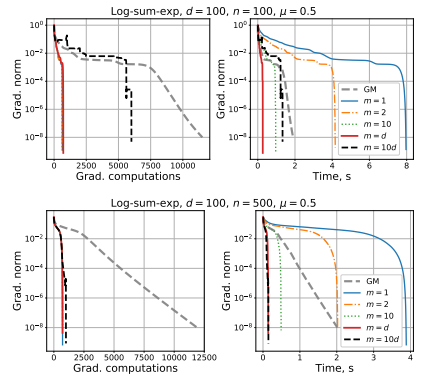
\includegraphics[width=0.8\textwidth]{figs/1.png}
    \caption{Hessian更新频率对算法性能的影响}
    \label{fig:fig1}
\end{figure}

实验结果表明:

1. 通过增加Hessian更新的频率(即增加$m$的值),可以显著提高算法的总体性能。最优的更新频率是 
$m=d$,这与理论分析一致。

2. 与每次迭代都更新Hessian矩阵的经典牛顿法相比,Lazy Hessian更新方法在保持收敛速度的同时,显著减少了计算成本。

3. 二阶方法(如立方牛顿法和正则化牛顿法)在收敛速度和计算效率上均优于经典的梯度法。



\newpage

\section{论文的结论}

在本文中,开发了新的带有\textbf{LazyHessian更新}的二阶优化算法,用于解决一般的非凸优化问题。展示了在多次迭代中重用先前计算的Hessian矩阵可以显著提高算法的效率,而不需要每次迭代都更新Hessian矩阵。

通过使用\textbf{立方正则化}和\textbf{梯度正则化}技术,证明了带有LazyHessian更新的二阶方法在广泛的凸和非凸优化问题中具有快速的全局和局部收敛速度。证明了最优的Hessian更新策略是每 \(d\) 次迭代更新一次Hessian矩阵,其中 \(d\) 是问题的维度。这显著减少了二阶算法的总算术复杂度,提高了 \(\sqrt{d}\) 倍。

\section{未来可行的研究}
\begin{enumerate}
    \item \textbf{特定Hessian结构的研究}:研究具有特定Hessian结构(如稀疏性或某些谱聚类)的问题,可能需要不同的Hessian更新策略。
    \item \textbf{与拟牛顿法的联系}:探索LazyHessian更新与经典拟牛顿法之间的联系。拟牛顿法通过逐步更新Hessian矩阵的近似来优化问题。
    最近发现的拟牛顿法的非渐近复杂度界限(Rodomanov \& Nesterov, 2021; Rodomanov, 2022)可能对实现这一目标特别有用。
    \item \textbf{高阶优化方案的推广}:将分析推广到高阶优化方案(Nesterov, 2021)。高阶方法使用更高阶的导数信息来加速收敛。
	主要挑战是如何高效地重用高阶张量,这可能需要使用一些高级的张量分解技术。
    \item \textbf{凸优化的进一步研究}:在凸优化中,除了梯度范数外,另一个常见的精度度量是函数残差。
	可能可以证明使用函数残差作为度量时,LazyHessian更新方法具有更好的收敛速度。还可以研究加速和超通用的二阶方法。
\end{enumerate}
\newpage


\section{参考}\label{section:related}
参考凸优化教材牛顿迭代法部分内容\cite{nesterov2013introductory}
% 在相关工作以及其他任何章节,我们可以引用文献来说明相关的工作。

% {\color{blue}
% 例如,我们可以如下撰写。
% 在\citeyear{nesterov2013introductory}年,\citeauthor{nesterov2013introductory}
% 撰写了关于凸优化基本原理的教材\cite{nesterov2013introductory}。此后,
% 一种简单的有限和最小化问题的简单加速算法被提出\cite{defazio2016simple},
% 成为多种算法的基础\cite{eisen2017decentralized,davis2015convergence,colin2016gossip}。
% %
% 由于算力的紧张,将优化计算分布在多个不同的计算节点上,成为优化领域的新方向。
% 主要方法可以粗略地分为两条技术路线。第一条技术路线的代表性工作是DFISTA\cite{wu2016decentralized}...
% }




% %+++++++++++++++++++++++++++++++++++++++++++++++++++++++++++++++++++++++++++++
% % Bibliography
% %+++++++++++++++++++++++++++++++++++++++++++++++++++++++++++++++++++++++++++++
\bibliographystyle{gbt7714-plain}
\bibliography{main}

%+++++++++++++++++++++++++++++++++++++++++++++++++++++++++++++++++++++++++++++
\end{document}
%+++++++++++++++++++++++++++++++++++++++++++++++++++++++++++++++++++++++++++++


